\begin{parag}{How to show this formula? (Outbook)}
    Let us extend $f: \mathbb{R}_+ \to \mathbb{C}$ to a function defined on $ \mathbb{R}$ by setting it to be $0$ on $\left(-\infty, 0\right)$. Let us define 
	\begin{align*} 
		g\left(t\right) =  f\left(t\right)e^{-\gamma t}
	\end{align*}
	And let us take the Fourier transform of $g$
	\begin{align*} 
		\hat{g}\left(a\right) &= \frac{1}{\sqrt{2\pi}} \int_{-\infty}^{\infty}g\left(t\right)e^{-iat}dt \\
		&= \frac{1}{\sqrt{2\pi}}\int_{-\infty}^{\infty}f\left(t\right)e^{-\left(\gamma + ia\right)t}dt \\
		&= \frac{1}{\sqrt{2\pi}}\int_{0}^{\infty}f\left(t\right)e^{-\left(\gamma + ia\right)t}dt = \mathcal{L}\left[f\right]\left(\gamma + ia\right)
	\end{align*}
	Now let us take the inverse of the Fourier transform 
	\begin{align*} 
		g\left(t\right) &=  \frac{1}{\sqrt{2\pi}} \int_{-\infty}^{\infty}\hat{g}\left(a\right)e^{iat}da \\
		&= \frac{1}{2\pi} \int_{-\infty}^{\infty}F\left(\gamma + ia\right)e^{iat}da\\
		&\implies f\left(t\right) =  e^{\gamma t}g\left(t\right) = \frac{1}{2\pi}\int_{-\infty}^{\infty}F\left(\gamma + ia\right)e^{\left(\gamma + ia\right)t}dt
	\end{align*}
\end{parag}
\begin{framedremark}
	\begin{enumerate}
	    \item Lercle's theorem tells us that $f$ is uniquely determined by $\mathcal{L}\left[f\right]$ through this formula
	    \item The condition $\lim_{T \to \infty} \int_{-T}^{T}F\left(\gamma + is\right)e^{\left(\gamma + is\right)t}ds < \infty$ is given when provided that 
			\begin{align*} 
				\int_{-\infty}^{\infty}\left|F\left(\gamma + is\right)\right|ds < \infty
			\end{align*}
	\end{enumerate}

\end{framedremark}


\paragraph{Example}%
\label{par:ExampleInverse}
    Let us have the function 
	\begin{align*} 
		F\left(z\right) = \frac{1}{\left(z + 1\right)\left(z + 2\right)^2}
	\end{align*}
	The goal is to find a $f: \mathbb{R}_+ \to \mathbb{C}$ such that $\mathcal{L}\left[f\right] = F$. To do so we have two ways.

\begin{parag}{Partial fraction decomposition}
	Using partial fraction decomposition, we can simplify our function into a sum of easier function 
	\begin{align*} 
		\frac{1}{\left(z + 1\right)\left(z + 2\right)^2} = \underbrace{\frac{1}{z+1}}_{= \mathcal{L}\left[e^{-t}\right]} - \underbrace{\frac{1}{z + 2}}_{= \mathcal{L}\left[e^{-2t}\right]} -\underbrace{\frac{1}{\left(z + 2\right)^2}}_{= \mathcal{L}\left[t e^{-2t}\right]} 
	\end{align*}
	And as the inverse of the Laplace transform of those function is known/ easy to find we get 
    \begin{align*} 
		f\left(t\right) = e^{-t} - e^{-2t} -te^{-2t}
	\end{align*}
	And by \important{uniqueness} of the Laplace transform, this is enough to find $f$ and it usually is the fastest way.
\end{parag}


\begin{parag}{Inverse Laplace transform and residue theorem}
	Using the inverse Laplace transform we know that $f$ is given as 
	\begin{align*} 
		f\left(t\right) = \frac{1}{2\pi} \int_{-\infty}^{\infty}F\left(\gamma + is\right)e^{\left(\gamma + is\right)t}ds
	\end{align*}
	Let $h\left(z\right) = F\left(z\right)e^{zt}$. The poles of our function $h$ are $z= =1$ and $z= -2$. For simplicity, let us choose $\gamma = 0$. Now we have to check some properties before we can actually compute this integral, we have that 
	\begin{enumerate}
	    \item $F$ is holomorphic on $\left\{\text{Re }z > -1\right\}$
	    \item $\int_{-\infty}^{\infty}\left|F\left(\gamma + is\right)\right|ds < \infty$
	\end{enumerate}
	We have then the Inverse of the Laplace transform is given as 
	\begin{align*} 
		f\left(t\right) = \frac{1}{2\pi} \int_{-\infty}^{\infty}h\left(\gamma + is\right)ds = \frac{1}{2\pi i}\int_{-\infty i}^{\infty i}h\left(z\right)dz
	\end{align*}
	Now we can use our usual trick of closing the curve in order to be able to use the residue theorem. As our residue are on the left side of the complex plane, let us use the half circle which is defined on the left\\
	$ $\\
	To do so we will define two curves 
		\[\begin{split}
		L_r: \left[-r, r\right] &\longmapsto \mathbb{C} \\
		s &\longmapsto si
		\end{split}\]
		\[\begin{split}
		C_r: \left[\frac{\pi}{2}, \frac{2\pi}{2}\right] &\longmapsto \mathbb{C} \\
		\theta &\longmapsto re^{i\theta}
		\end{split}\]
	\begin{center}
	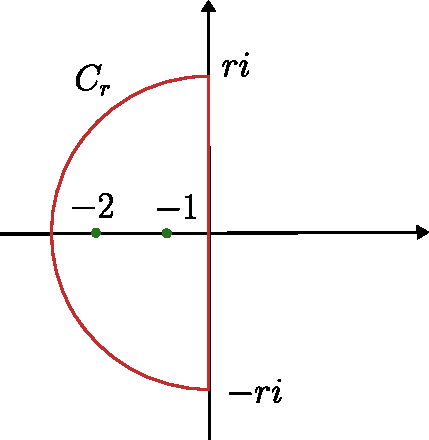
\includegraphics[width=0.4\textwidth]{figure/2026-05-08.pdf}
	\end{center}
	This gives us the curve $\Gamma$ we need as 
	\begin{align*} 
		\Gamma =  L_r \cup C_r \mathspace \text{ oriented counterclockwise}
	\end{align*}
	When $r > 2$, $\Gamma$ encloses all pole of $h$, namely $-1, -2$. Therefore now that we have done all the work (almost) to use the residue theorem, let us use it!
	\begin{align*} 
		\int_{\Gamma} h\left(z\right)dz =  2\pi i \left[\text{Res}_{-1}\left(h\right) + \text{Res}_{-2}\left(h\right)\right]
	\end{align*}
	Let us now computes the residue, the easiest one is $z =  -1$ as it is a simple pole. We therefore only need to compute the limit given as 
	\begin{align*} 
		\text{Res}_{-1}\left(h\right) = \lim_{z \to -1} \left(\left(z + 1\right)h\left(z\right)\right) = \lim_{z \to -1} \frac{e^{zt}}{\left(z + 2\right)^2} = e^{-t}
	\end{align*}
	For the second pole, $z = -2$ this pole is of order $2$ which therefore implies that we need to take the derivative as 
	\begin{align*} 
		\text{Res}_{-2}\left(h\right) &= \lim_{z \to -2} \frac{d}{dz} \left(z + 2\right)^2 h\left(z\right)\\
		&= \lim_{z \to -2}  \frac{d}{dz} \left(\frac{e^{zt}}{z + 1}\right) = -e^{-zt}\left(t + 1\right)
	\end{align*}
	Hence giving us the result 
	\begin{align*} 
		\int_{\Gamma} h\left(z\right) dz = 2\pi i \left[e^{t} - e^{-2t} - te^{-2t}\right]
	\end{align*}
	What we need to show now is that the $L_r$ part of the integral vanishes as $r \to \infty$, to do so we will use a bit of triangle inequality everywhere. The goal is to show that the integral 
	\begin{align*} 
		\left|\int_{C_r} h\left(z\right)dz\right| \to 0 \text{ as }r \to \infty
	\end{align*}

	\begin{align*} 
		\left|\int_{C_r}h\left(z\right)dz\right| &= \left|\int_{\frac{\pi}{2}}^{\frac{3\pi}{2}}g\left(re^{i\theta}\right)ire^{i\theta}d \theta\right|\\
												 &\leq \int_{\frac{\pi}{2}}^{\frac{3\pi}{2}}\left|h\left(re^{i\theta}\right)\right|rd \theta\\
												 &= \int_{\frac{\pi}{2}}^{\frac{3\pi}{2}}\frac{\left|e^{re^{i\theta}}\right|}{\left|re^{i\theta} + 1\right|\left|re^{i\theta} + 2\right|^2}r d \theta
	\end{align*}
	And here we can noting that the term $r \cdot  \cdots$ dominates, the lower term of this integral can be approximates by $\sim r \cdot \sim r^2$. Now let us work with the upper term 
	\begin{align*} 
		\left|e^{re^{i\theta}}\right| &= \left|e^{r\left(\cos \theta + i \sin \theta\right)t}\right|\\
		&= \left|e^{r \cos \theta t}\right|\left|\underbrace{e^{ir\sin \theta t}}_{= 1}\right|= e^{r \cos \theta t} \leq 1
	\end{align*}
	Because $\cos \theta \leq 0$ for $\theta \in \left[\frac{\pi}{2}, \frac{3\pi}{2}\right]$. Hence, the integral $\left|\int_{C_r}h\left(z\right)dz\right|$ can be bounded from above by a term of order 
	\begin{align*} 
		\int_{\frac{\pi}{2}}^{\frac{3\pi}{2}} \frac{1}{r r^2}r d \theta \to 0 \text{ as } r \to \infty
	\end{align*}
	Therefore, we have found our inverse given as 
	\begin{align*} 
		\frac{1}{2\pi i} \cdot  2\pi i\left[e^{t} - e^{-2t} - te^{-2t}\right]
	\end{align*}

\end{parag}


\begin{framedremark}
	We chose the left half circle (for $\text{Re } z < \gamma$) because in that region $\left|e^{zt}\right| \leq e^{\gamma t}$. This guarantees the control on the upper term of $h$.
\end{framedremark}


\section{Application to partial differential equations (PDES)}
As for ODES we will apply the theory of Laplace and Fourier transform to solve initial boundary value problems for linear partial differential equations with constant coefficients, e.g. heat equation 

\begin{align*} 
	\frac{\partial u}{\partial t} \left(x, t\right) - \frac{\partial^2 u}{\partial x^2} u\left(x, t\right) = f\left(x, t\right)
\end{align*}
For $t > 0$ and $x \in \left(0, L\right)$. We stipulate (or give the initial condition)
\begin{align*} 
	u\left(x, 0\right) &= u_0\left(x\right)\\
	u\left(0, t\right) &= u\left(L, t\right) = 0 \mathspace \text{ boundary condition}
\end{align*}
It describes the evolution of temperature $u$ of a one dimensional rod of length $L$ with a heat source $f$ and fixed temperature at endpoints $0, L$.\\
$ $\\
Let us before starting summarize the general procedure that we will follow. There is three different '\textit{tools}' that we can use:
\begin{itemize}
    \item \important{Fourier series} if the space or time domain is bounded
    \item \important{Fourier transform} if the space or time domain is on $ \mathbb{R}$
    \item \important{Laplace transform} if the space or time domain is half unbounded ($ \mathbb{R}_+$)
\end{itemize}

\subsection{Recall of Fourier series}
What we want to decompose is a function $f: \left[0, L\right] \to \mathbb{R}$ into an infinite sum of oscillating functions. Those function are made using \important{basis function}, namely 
\begin{align*} 
	\sin\left(\frac{2\pi n}{L}x\right) \mathspace \text{ where }n \geq 1 \\
	\cos \left(\frac{2\pi n}{L}x\right) \mathspace \text{ where }n \geq 0
\end{align*}


\begin{parag}{Orthogonality}
	\begin{definition}{Inner product}
    The inner product between two function $f, g$ is given as 
	\begin{align*} 
		< f, g> := \int_{0}^{L}f\left(x\right)g\left(x\right) dx
	\end{align*}
	\end{definition}
	\begin{align*} 
		< \sin\left(\frac{2\pi n}{L}x\right), \sin\left(\frac{2\pi n}{L}x\right)> =  \begin{cases}
		\frac{L}{2} \mathspace \text{ if } m = n\\
			0 \mathspace \text{ otherwise}
		\end{cases}	\end{align*}
		The same foes for the product 
		\begin{align*} 
			< \cos\left(\frac{2\pi n}{L}x\right), \cos \left(\frac{2\pi n}{x}\right)>
		\end{align*}
		\begin{theoreme}
		\begin{align*} 
			<\sin\left(\frac{2\pi n}{L}x\right), \cos \left(\frac{2\pi n}{L}x\right)> =  0 \mathspace \forall n, m
		\end{align*}
		\end{theoreme}
		As we can see those function creates an orthogonal basis which we can use in order to decompose other function. \\
		$ $\\
		The question that the Fourier series is answering is: Given $f: \left[0, 1\right] \to \mathbb{R}$ be a piecewise continuous function, can we write it as 
		\begin{align*} 
			f\left(x\right) = \frac{a_0}{2} + \sum_{n = 1}^{\infty}\left[a_n \cos\left(\frac{2\pi n}{L}x\right) + b_n \sin\left(\frac{2\pi n}{L}x\right)\right]
		\end{align*}
		\begin{subparag}{Remark}
		    The same consideration apply when $f: \mathbb{R} \to \mathbb{R}$ is $L$-periodic, which can therefore be thought of as a function on $\left[0, L\right]$.
		\end{subparag}
\end{parag}






\begin{parag}{Coefficient of the serie}
    In order to guess the form of the coefficients $a_n$ and $b_n$, we will assume that $f$ already has this form. Then we can formally compute the following using orthogonality
	\begin{align*} 
		\int_{0}^{L}f\left(x\right)dx &= \frac{L}{2}a_0\\
		\int_{0}^{L}f\left(x\right)\cos\left(\frac{2\pi n}{L}x\right)dx &= \frac{L}{2}a_{n} \mathspace \text{ where } n\geq 1\\
		\int_0^{L}f\left(x\right)\sin\left(\frac{2\pi n}{L}x\right)dx &= \frac{L}{2}b_n \mathspace \text{ where } n \geq 1
	\end{align*}
	This suggests to define our coefficients as 
	\begin{align*} 
		a_n &= \frac{2}{L}\int_{0}^{L}f\left(x\right)\cos\left(\frac{2\pi n}{L}x\right)dx \mathspace \text{ where } n \geq0\\
		b_n &= \frac{2}{L}\int_{0}^{L}f\left(x\right)\sin\left(\frac{2\pi n}{L}x\right)dx \mathspace \text{ where } n\geq 1 
	\end{align*}

	\begin{theoreme}
	Define $f_N : \left[0, L\right] \to \mathbb{R}$ as 
	\begin{align*} 
		f_N \left(x\right) =  \frac{a_0}{2} + \sum_{n = 1}^{N}\left[a_n \cos\left(\frac{2\pi n}{L}x\right) + b_n \sin\left(\frac{2\pi n}{L}x\right)\right]
	\end{align*}
	Where $a_n$ and $b_n$ are defined as above, where $f: \left[0, L\right] \to \mathbb{R}$ is piecewise continuous. Then 
	\begin{align*} 
		f_N\left(x\right) \to f\left(x\right) \text{ as } N \to \infty \mathspace \text{ at every } x \in \left[0, L\right]\\
		f_N\left(x\right) \to \frac{f\left(x +\right) + f\left(x - \right)}{2} \mathspace \text{ when } x \text{ is a jump discontinuity of }f\\
		\lim_{N \to \infty} \int_0^{L}\left|f_N\left(x\right) - f\left(x\right)\right|dx = 0
	\end{align*}
	\end{theoreme}
	The definition of the $f\left(x +\right)$ and $f\left(x -\right)$ are designed in such that when we have a discontinuity, we are effectively taking the mean of those two points
	\begin{center}
	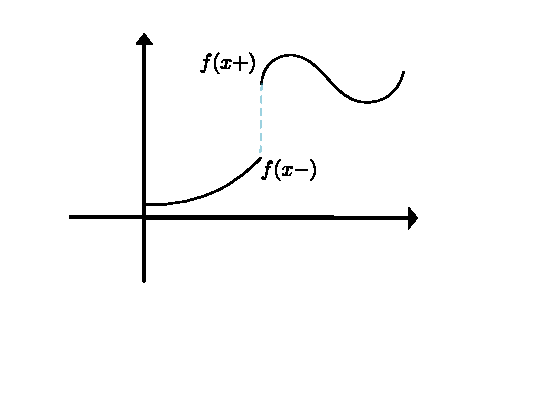
\includegraphics[width=0.7\textwidth]{figure/2026-05-07_1.pdf}
	\end{center}
\end{parag}


\begin{parag}{Special cases}
	\begin{subparag}{$f$ is odd}
    Assume $f$ is odd, then 
	\begin{align*} 
		a_n = 0 \mathspace \forall n \geq 0 
	\end{align*}
	And therefore 
	\begin{align*} 
		f\left(x\right) = \sum_{n= 1}^{\infty}b_n \sin\left(\frac{2\pi n}{L}x\right)
	\end{align*}
	Where 
	\begin{align*} 
		b_n &= \frac{2}{L}\int_0^{L}f\left(x\right) \sin\left(\frac{2\pi n}{L}x\right)dx\\
			&=  \frac{2}{L} \int_{-\frac{L}{2}}^{\frac{L}{2}}f\left(x\right) \sin\left(\frac{2\pi n}{L}x\right)dx\\
			&= \frac{4}{L}\int_0^{\frac{L}{2}}f\left(x\right)\sin\left(\frac{2\pi n}{L}x\right)dx
	\end{align*}
	We are able to do so as $f$ and $\sin$ are odd, their product is even.
	\end{subparag}
	\begin{subparag}{$f$ is even}
	    Assume $f$ is even, then 
		\begin{align*} b_n = 0 \mathspace \forall n\geq 1 \end{align*}
		In this case $f$ is decomposed as
		\begin{align*} 
			f\left(x\right) = \frac{a_0}{2} + \sum_{n = 1}^{\infty}a_n \cos\left(\frac{2\pi n}{L}x\right)
		\end{align*}
		Where 
		\begin{align*} 
			a_n &= \frac{2}{L}\int_0^{L}f\left(x\right)\cos\left(\frac{2\pi n}{L}x\right)dx\\
				&= \frac{2}{L}\int_{-\frac{L}{2}}^{\frac{L}{2}}f\left(x\right)\cos\left(\frac{\pi n}{L}x\right)dx \mathspace \text{ by } L-\text{periodicity}\\
				&= \frac{4}{L}\int_{0}^{\frac{L}{2}}f\left(x\right)\cos\left(\frac{2\pi n}{L}x\right)dx
		\end{align*}
	\end{subparag}
	\begin{framedremark}
		\begin{itemize}
			\item The function $a_n \cos\left(\frac{2\pi n}{L}x\right)$ and $b_n \sin\left(\frac{2\pi n}{L}x\right)$ are sometimes called \important{modes}
			\item The function $e_n\left(x\right) = \cos\left(\frac{2\pi n}{L}x\right)$ satisfies the Neunmann boundary condition 
				\begin{align*} 
					e_n'\left(0\right)= 0 \mathspace e_n'\left(L\right)= 0
				\end{align*}
			\item The function $h_n\left(x\right) =  \sin\left(\frac{2\pi n}{L}x\right)$ satisfies \important{Dirichlet boundary conditions} 
				\begin{align*} 
					h_n\left(0\right) = 0 \mathspace h_n\left(L\right) = 0
				\end{align*}
		\end{itemize}
		
	\end{framedremark}
\end{parag}











